\documentclass[12pt]{article}
\usepackage[authoryear]{natbib}
\usepackage[english]{babel}
\usepackage{amsmath,amssymb}
\usepackage{ifthen}
\usepackage{graphicx}
\usepackage{amsthm}
\usepackage{epstopdf}
%\usepackage{commath}
\usepackage{hyperref}
%\usepackage{pstricks}
\usepackage{mathrsfs}
%\usepackage{csquotes}
\usepackage{amssymb}
\usepackage{amsfonts}
\usepackage{mathtools}
%\usepackage{makecell}
\usepackage{rotating}
\usepackage[font=small,labelfont=bf]{caption}
\usepackage{subcaption}
\usepackage{geometry}
\usepackage{setspace}
\usepackage{xr}
%\usepackage{bbm}
\usepackage{multirow}
\usepackage{enumitem}
%\usepackage[en-US]{datetime2}
\usepackage{color}
%\usepackage{csvsimple,booktabs}
%\usepackage{booktabs} % For formal tables
%\usepackage{fullpage}
%\usepackage[ruled,vlined]{algorithm2e}
%\usepackage{algorithm}
%\usepackage{algpseudocode}
%\usepackage[stable]{footmisc}
%\usepackage{pdfsync}

\newcommand{\E}{E}
%================================
% PATH

\graphicspath{{input/}{../../analysis/output}}

\newtheorem{theorem}{Theorem}
\newtheorem{fact}{Stylized Fact}
\newtheorem{corollary}{Corollary}[theorem]
\newtheorem{lemma}{Lemma}[section]
\newtheorem{proposition}{Proposition}
\theoremstyle{definition}
\newtheorem{defn}{Definition}
\newtheorem{step}{Step}
\newtheorem{remark}{Remark}[section]
\newtheorem{example-continued}{Example}
\newtheorem{example}{Example}
\newtheorem{assumption}{Assumption}
\newtheorem{cor}{Corollary}


\newcommand{\simon}[1]{\textcolor{olive}{\textbf{Simon: #1}}}
\newcommand{\chg}[1]{\textcolor{blue}{\textbf{#1}}}

\author{
        Simon Freyaldenhoven\\
        \textit{Federal Reserve Bank of Philadelphia\thanks{I thank Ryan Kobler for her help in setting up this template. The views expressed herein are those of the authors and do not necessarily reflect the views of the Federal Reserve Bank of Philadelphia, or the Federal Reserve System. Emails: \href{mailto:simon.freyaldenhoven@phil.frb.org}{simon.freyaldenhoven@phil.frb.org}}}
}
\title{A quick note}


\date{\today}

\begin{document}

\maketitle

\begin{abstract}
\noindent This note illustrates how a draft uses the output produced by the code under \texttt{/analysis/}
\end{abstract}

JEL-Classification: C..

\textsc{Keywords}: TBA

\thispagestyle{empty}
% \newpage
% \tableofcontents
% \thispagestyle{empty}
\newpage

\setcounter{page}{1}

\section{The only section}

\begin{itemize}
\item We use bibtex for references (e.g. \cite{Freyaldenhoven2019}). 

\item Ideally all numbers should be softcoded, and come directly from output. For example, in our baseline simulations setup, where we simulate the throw of two 6-sided dice, the average sum of the two throws is equal to \input{../../analysis/output/simulation/baseline/mean_sum.txt}\unskip. That way all numbers are by construction always up-to-date.

\item Below, Figure \ref{fig:hist_baseline} includes a histogram of the simulation exercise.
\end{itemize}
\begin{figure}[tbh!]
\centering
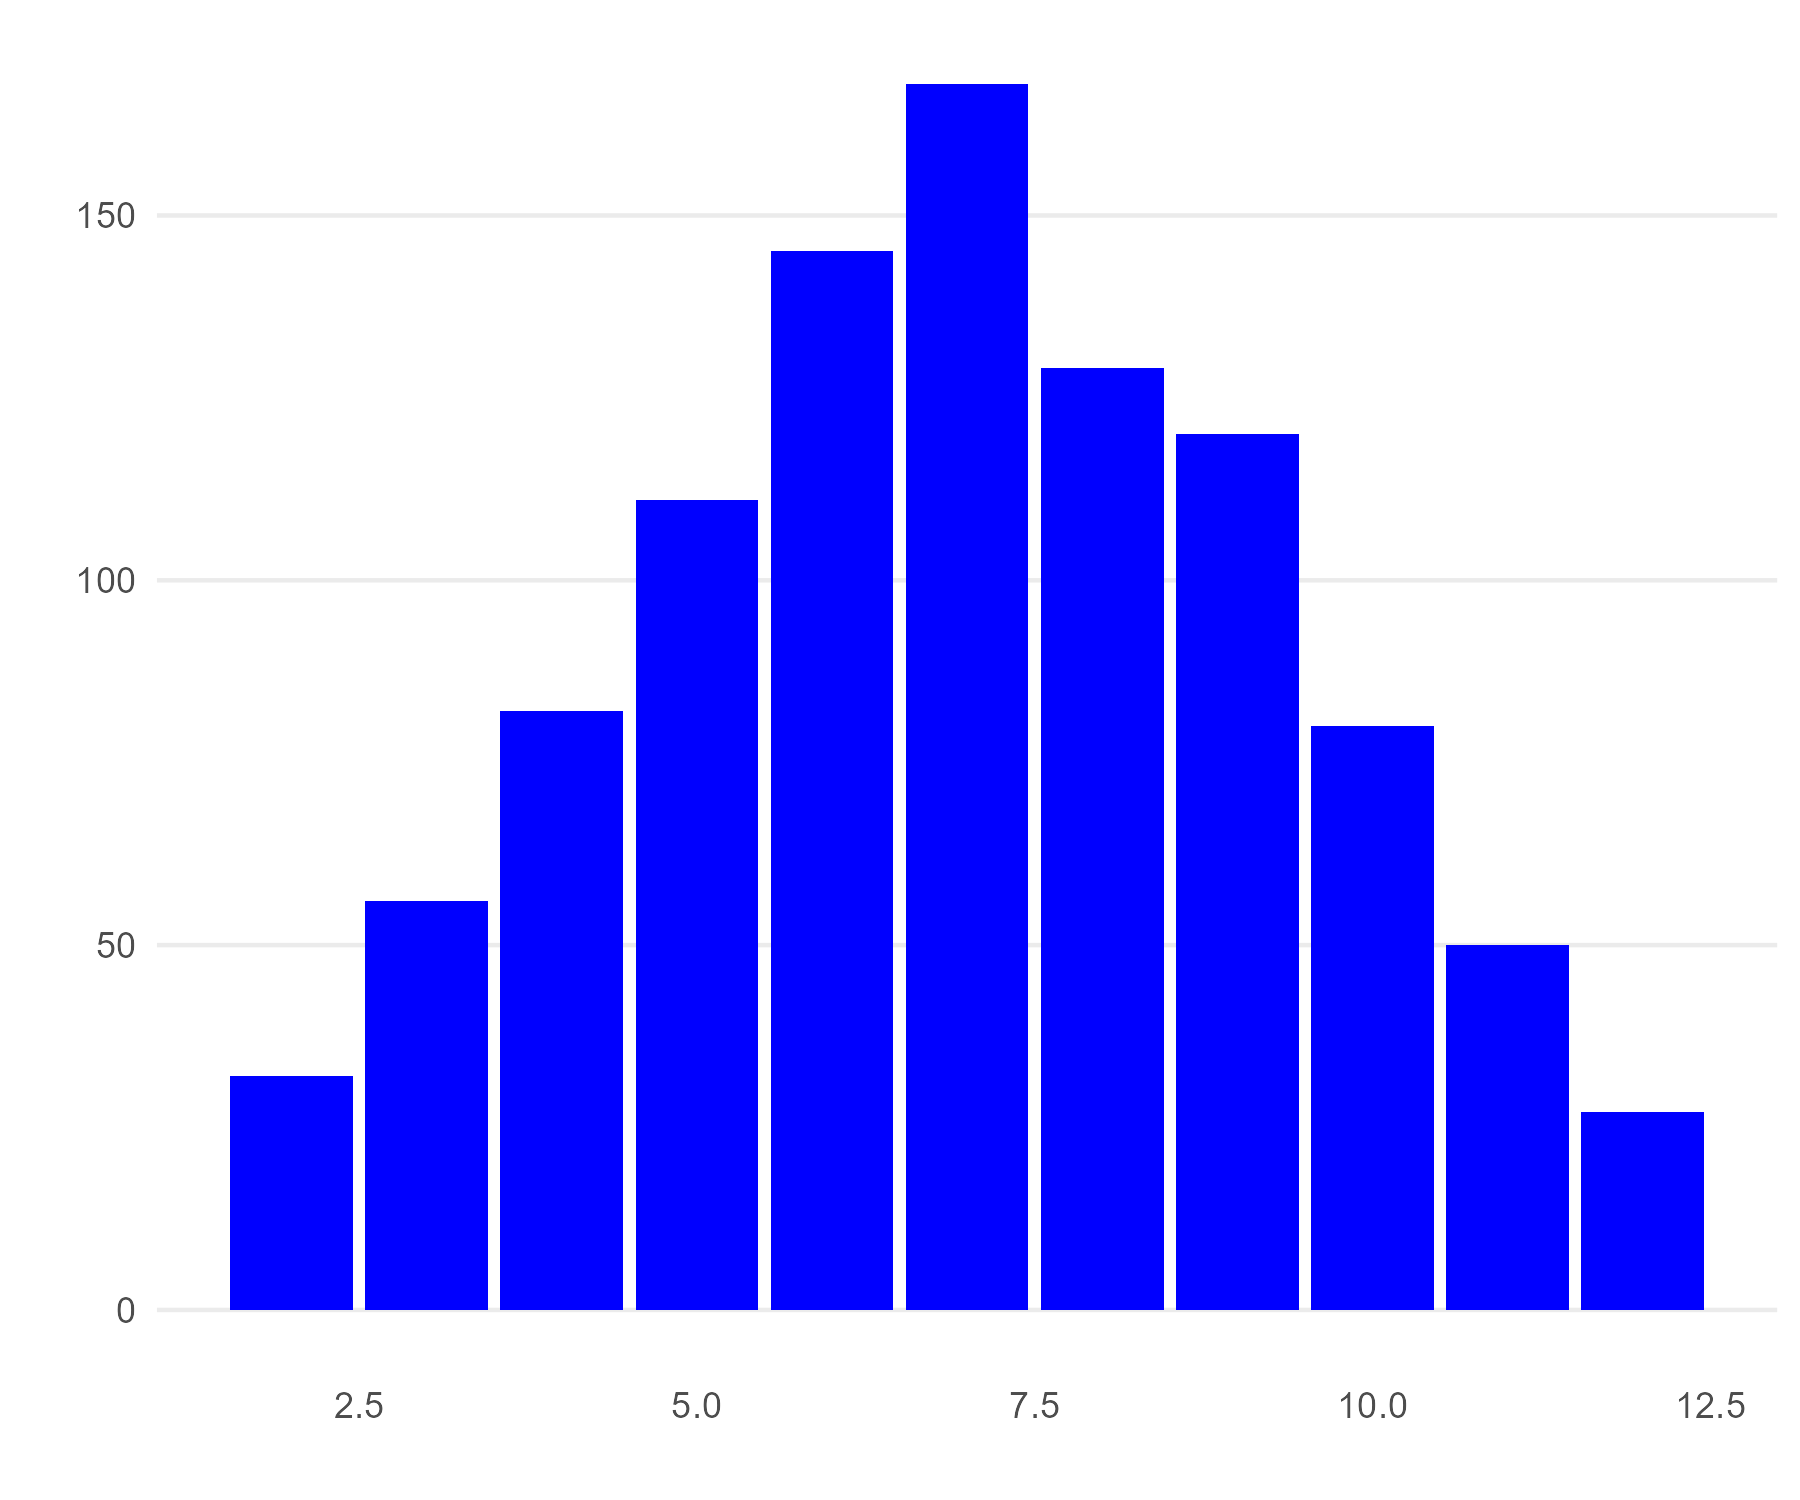
\includegraphics[width=.8\linewidth]{plot/baseline/hist.png}
\caption[]{Numerical frequency for the sum of two six-sided die. Figure based on \input{../../analysis/output/simulation/baseline/sample_size.txt}throws.}
\label{fig:hist_baseline}
\end{figure}

We also include a second simulation for an 8-sided dice, where the average sum of the two throws is equal to \input{../../analysis/output/simulation/500_8/mean_sum.txt}\unskip. The corresponding histogram is depicted in Figure \ref{fig:hist_500_8} 
\begin{figure}[tbh!]
\centering
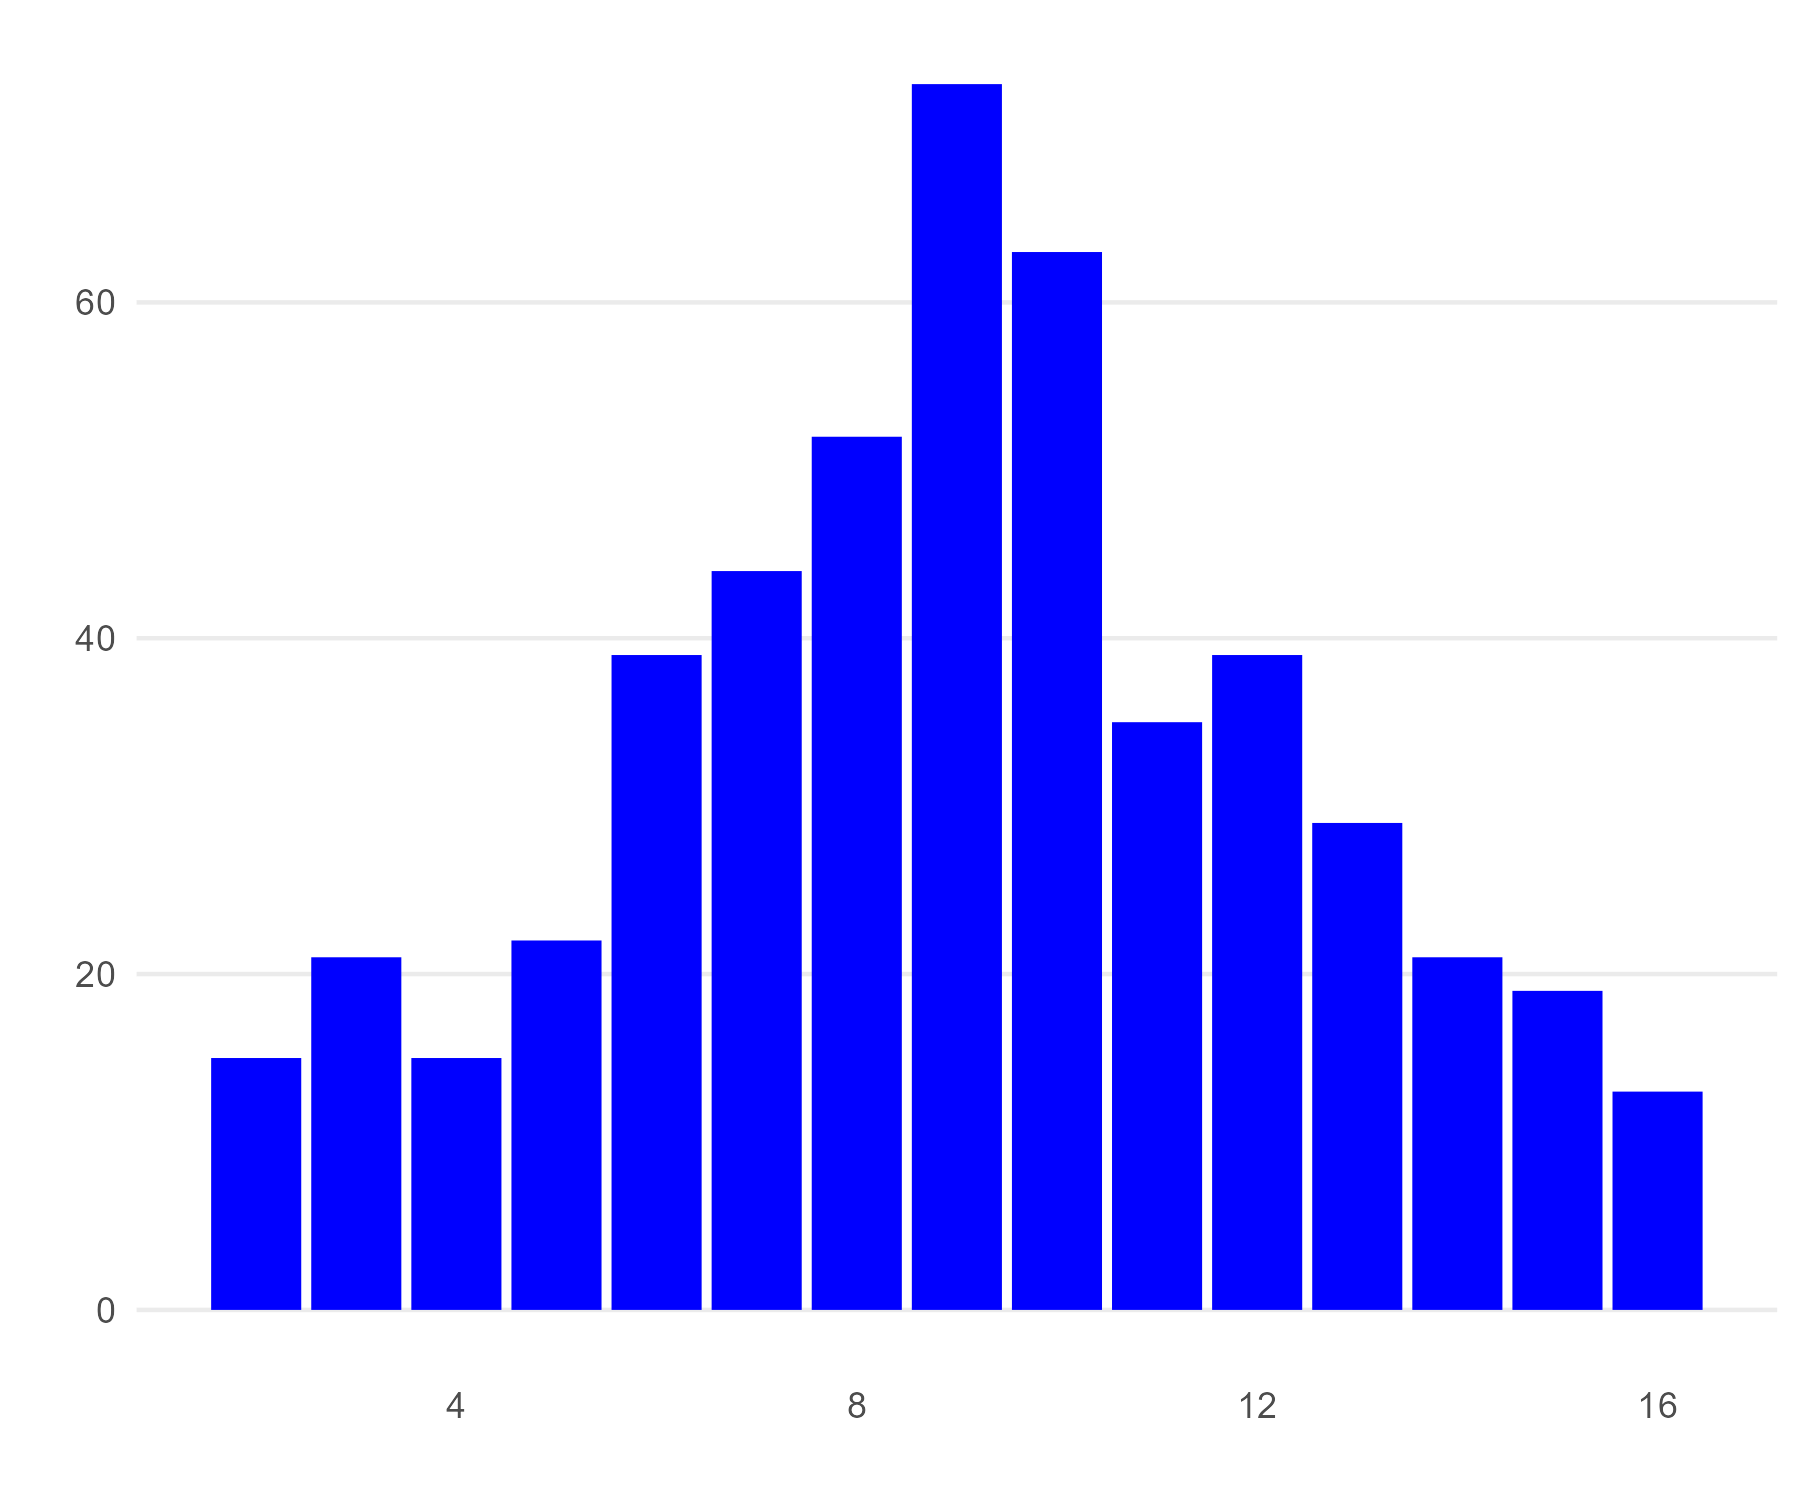
\includegraphics[width=.8\linewidth]{plot/500_8/hist.png}
\caption[]{Numerical frequency for the sum of two eight-sided die. Figure based on \input{../../analysis/output/simulation/500_8/sample_size.txt}throws.}
\label{fig:hist_500_8}
\end{figure}

\newpage

This is Figure \ref{fig:figsubplots} with both of the previous figures as subplots.
\begin{figure}[tbh!]
\begin{subfigure}{.4\textwidth}
  \centering
  % include first image
  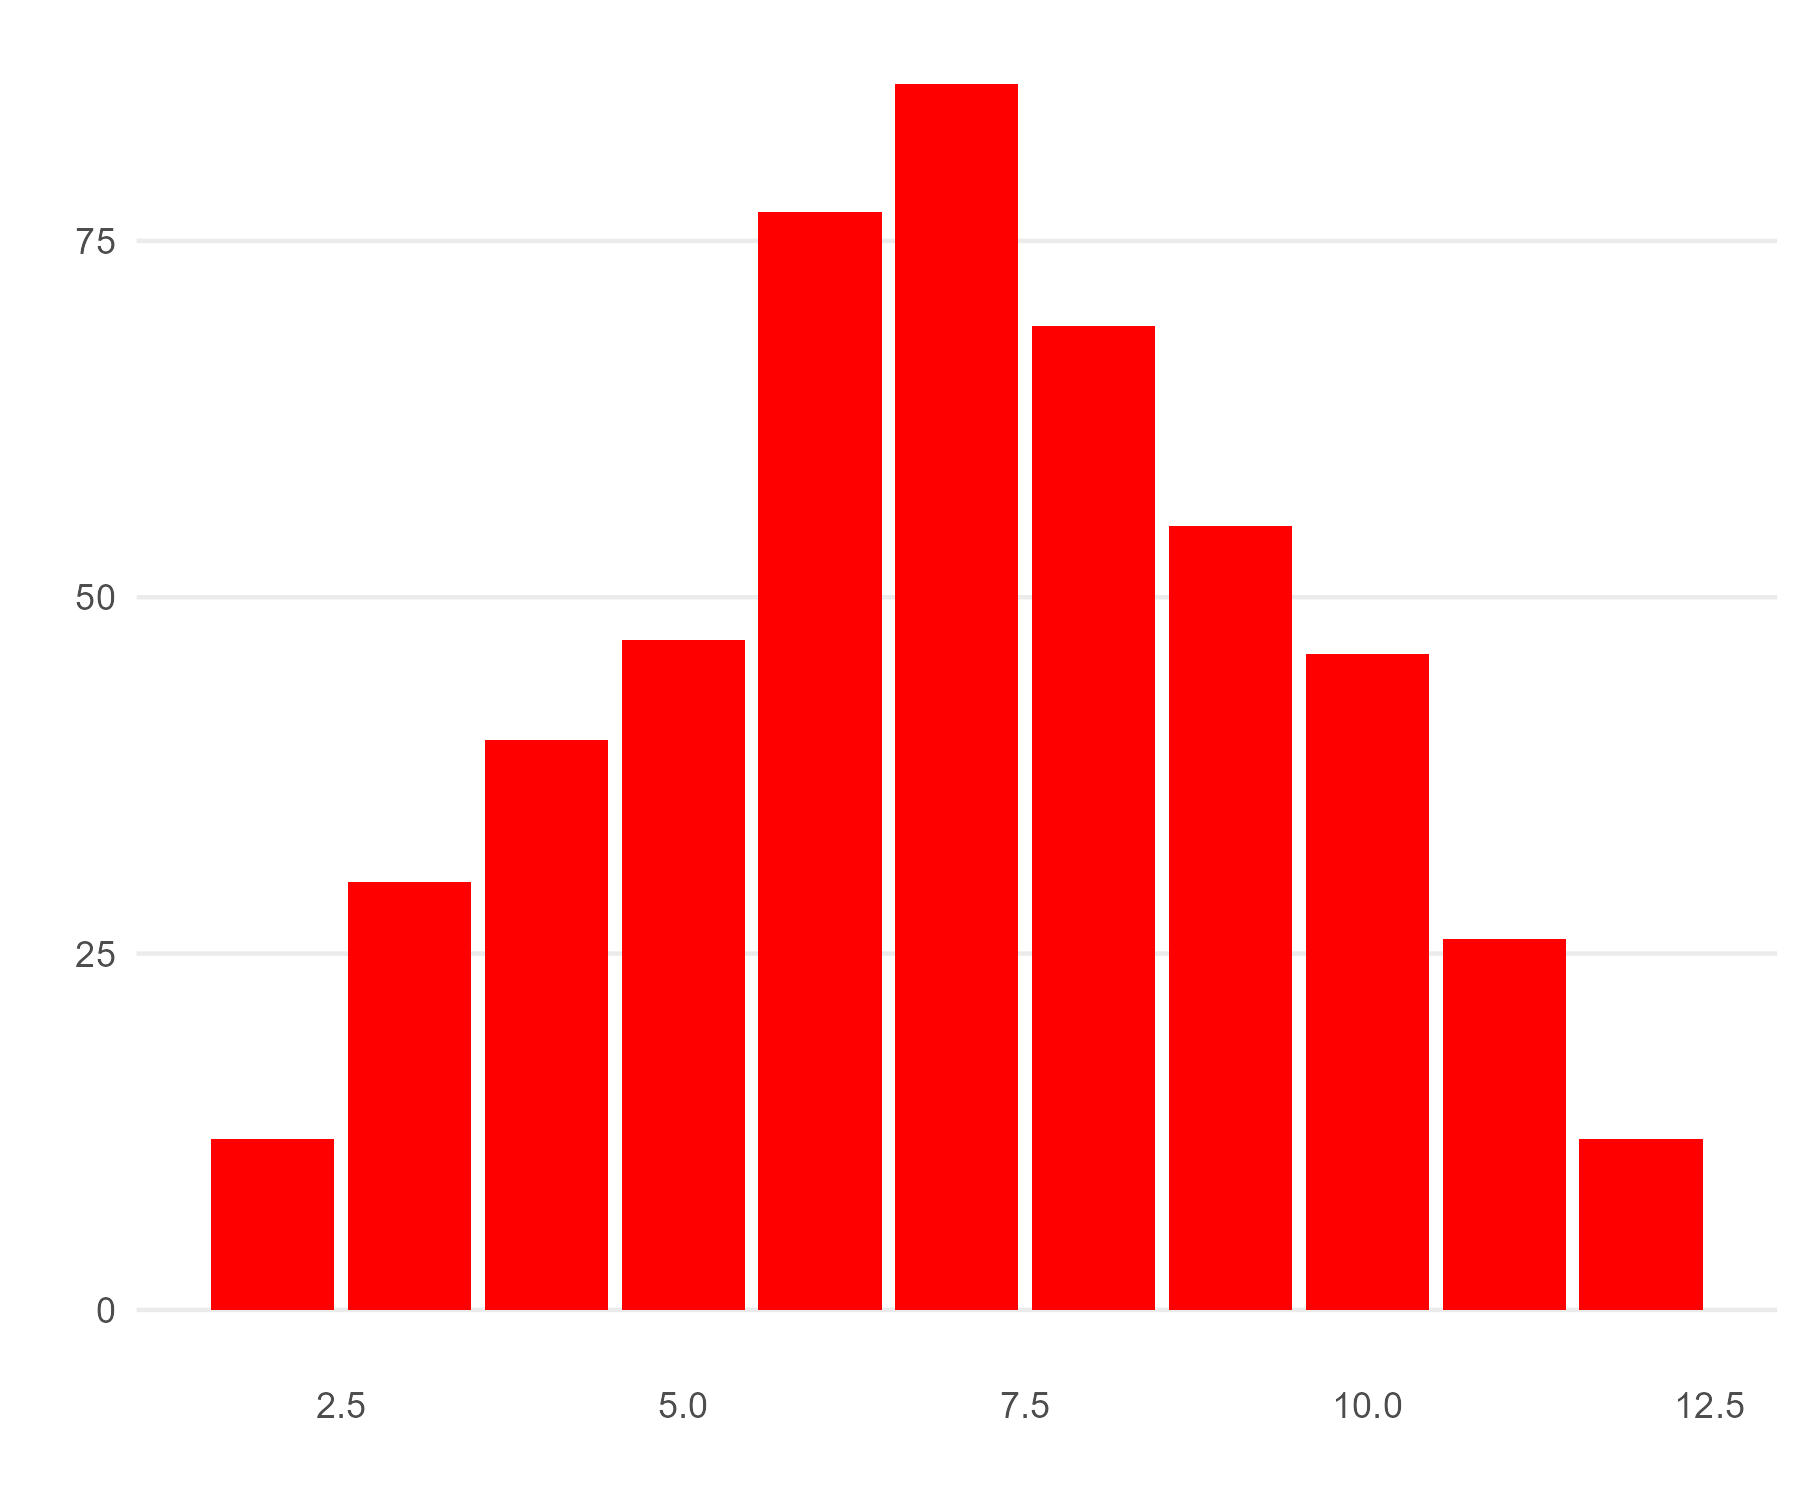
\includegraphics[width=.8\linewidth]{plot/baseline/hist_red.png}  
  \caption{Numerical frequency for the sum of two six-sided die. Figure based on \input{../../analysis/output/simulation/baseline/sample_size.txt}throws.}
  \label{fig:sub-first}
\end{subfigure}
\begin{subfigure}{.4\textwidth}
  \centering
  % include second image
  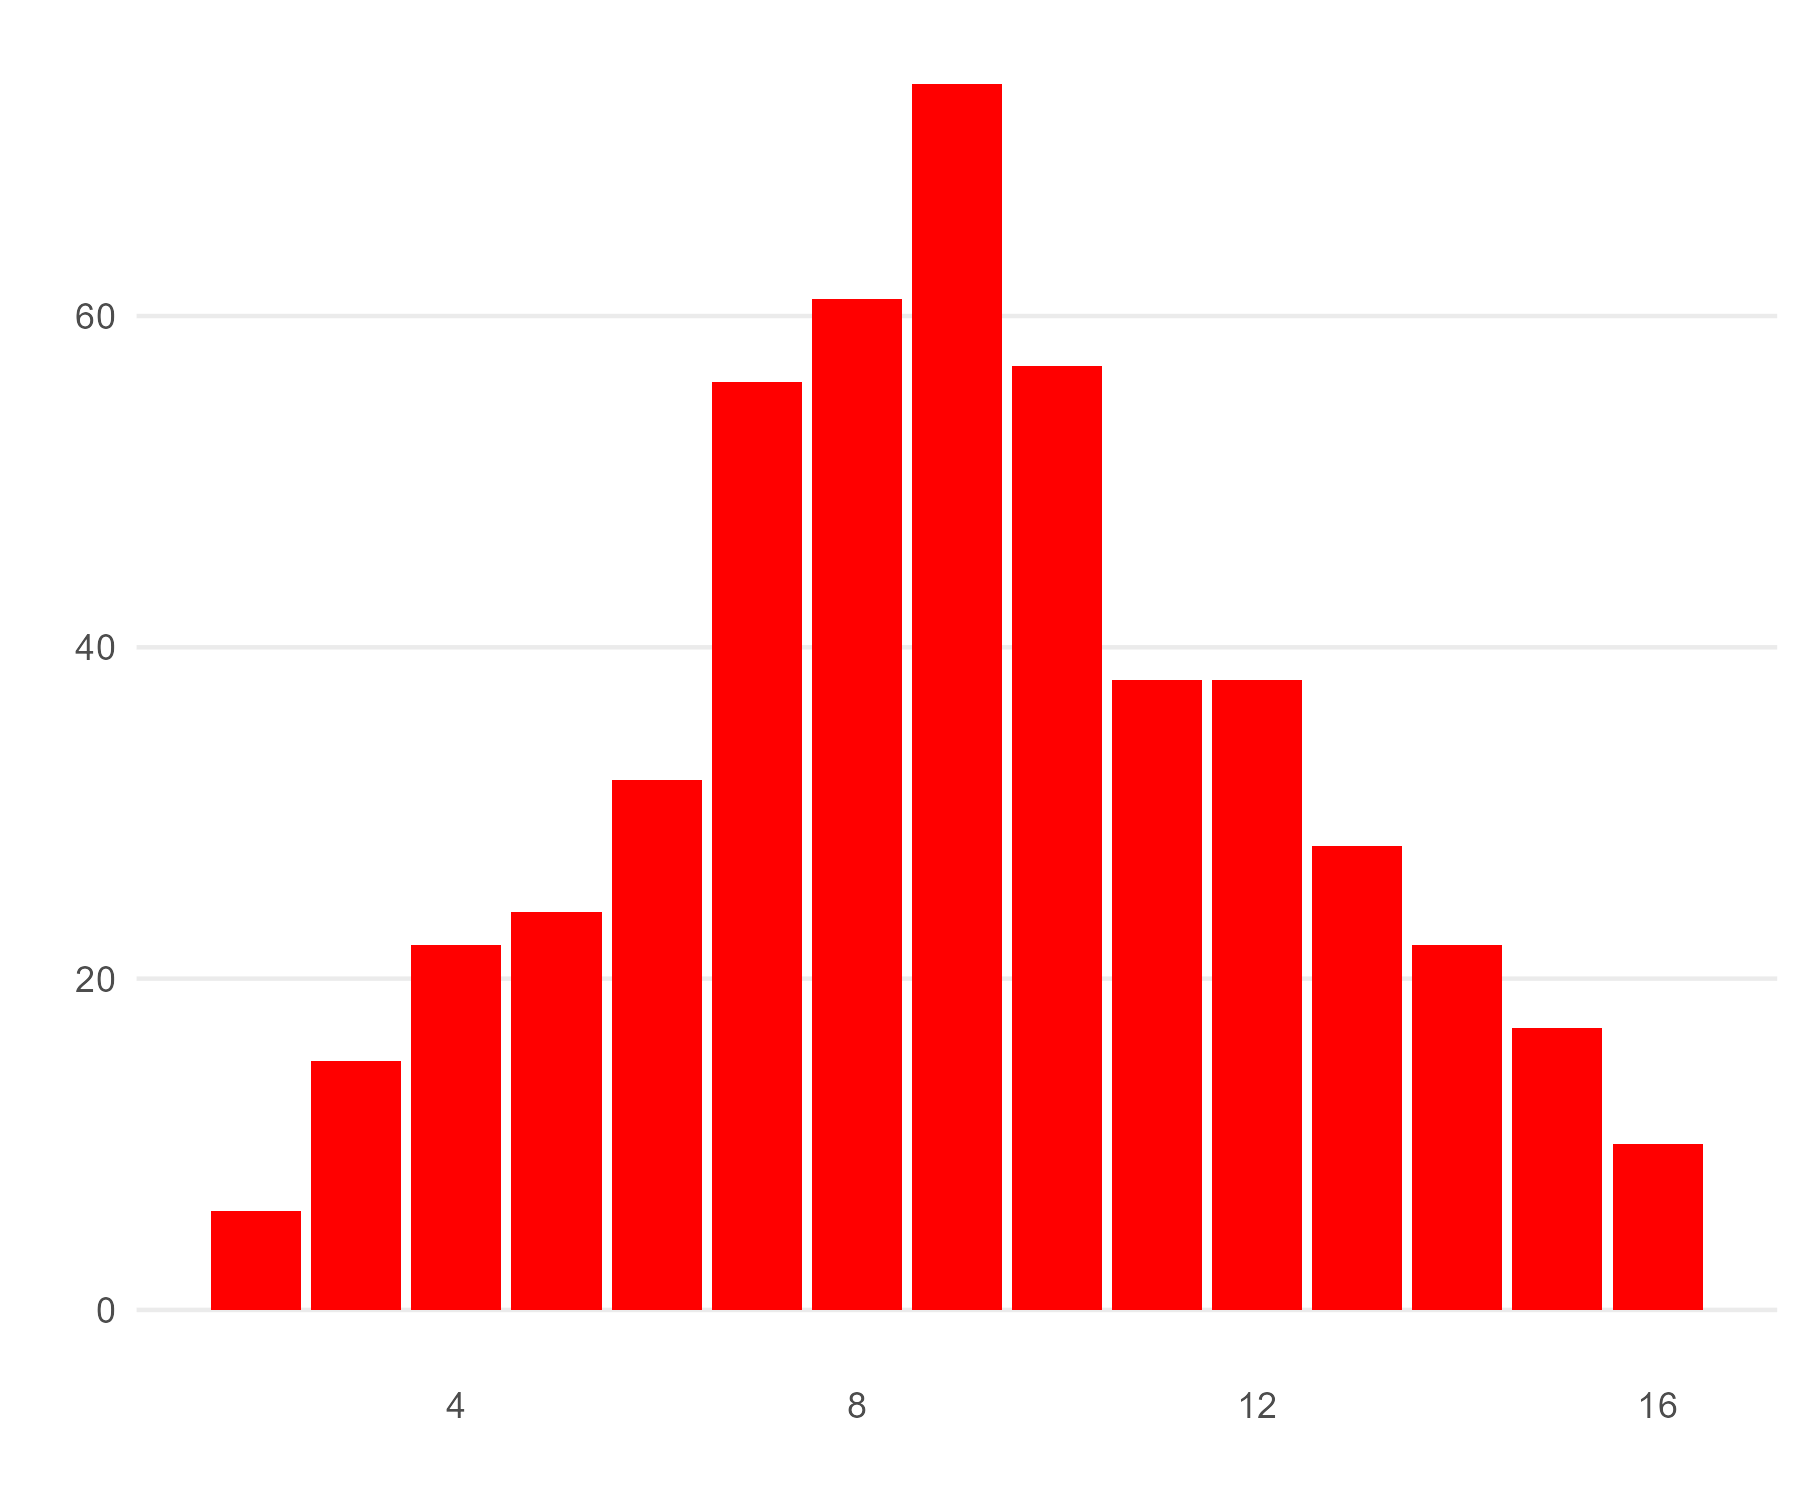
\includegraphics[width=.8\linewidth]{plot/500_8/hist_red.png}  
  \caption{Numerical frequency for the sum of two eight-sided die. Figure based on \input{../../analysis/output/simulation/500_8/sample_size.txt}throws.}
  \label{fig:sub-second}
\end{subfigure}
\caption{Combined plots of the simulations.}
\label{fig:figsubplots}
\end{figure}

\newpage

These are figures measuring the number of rolls by the current (total) sum over time. The first scatterplot, depicting rolls for two six-sided die is depicted in Figure \ref{fig:scatter_baseline} 
\begin{figure}[tbh!]
\centering
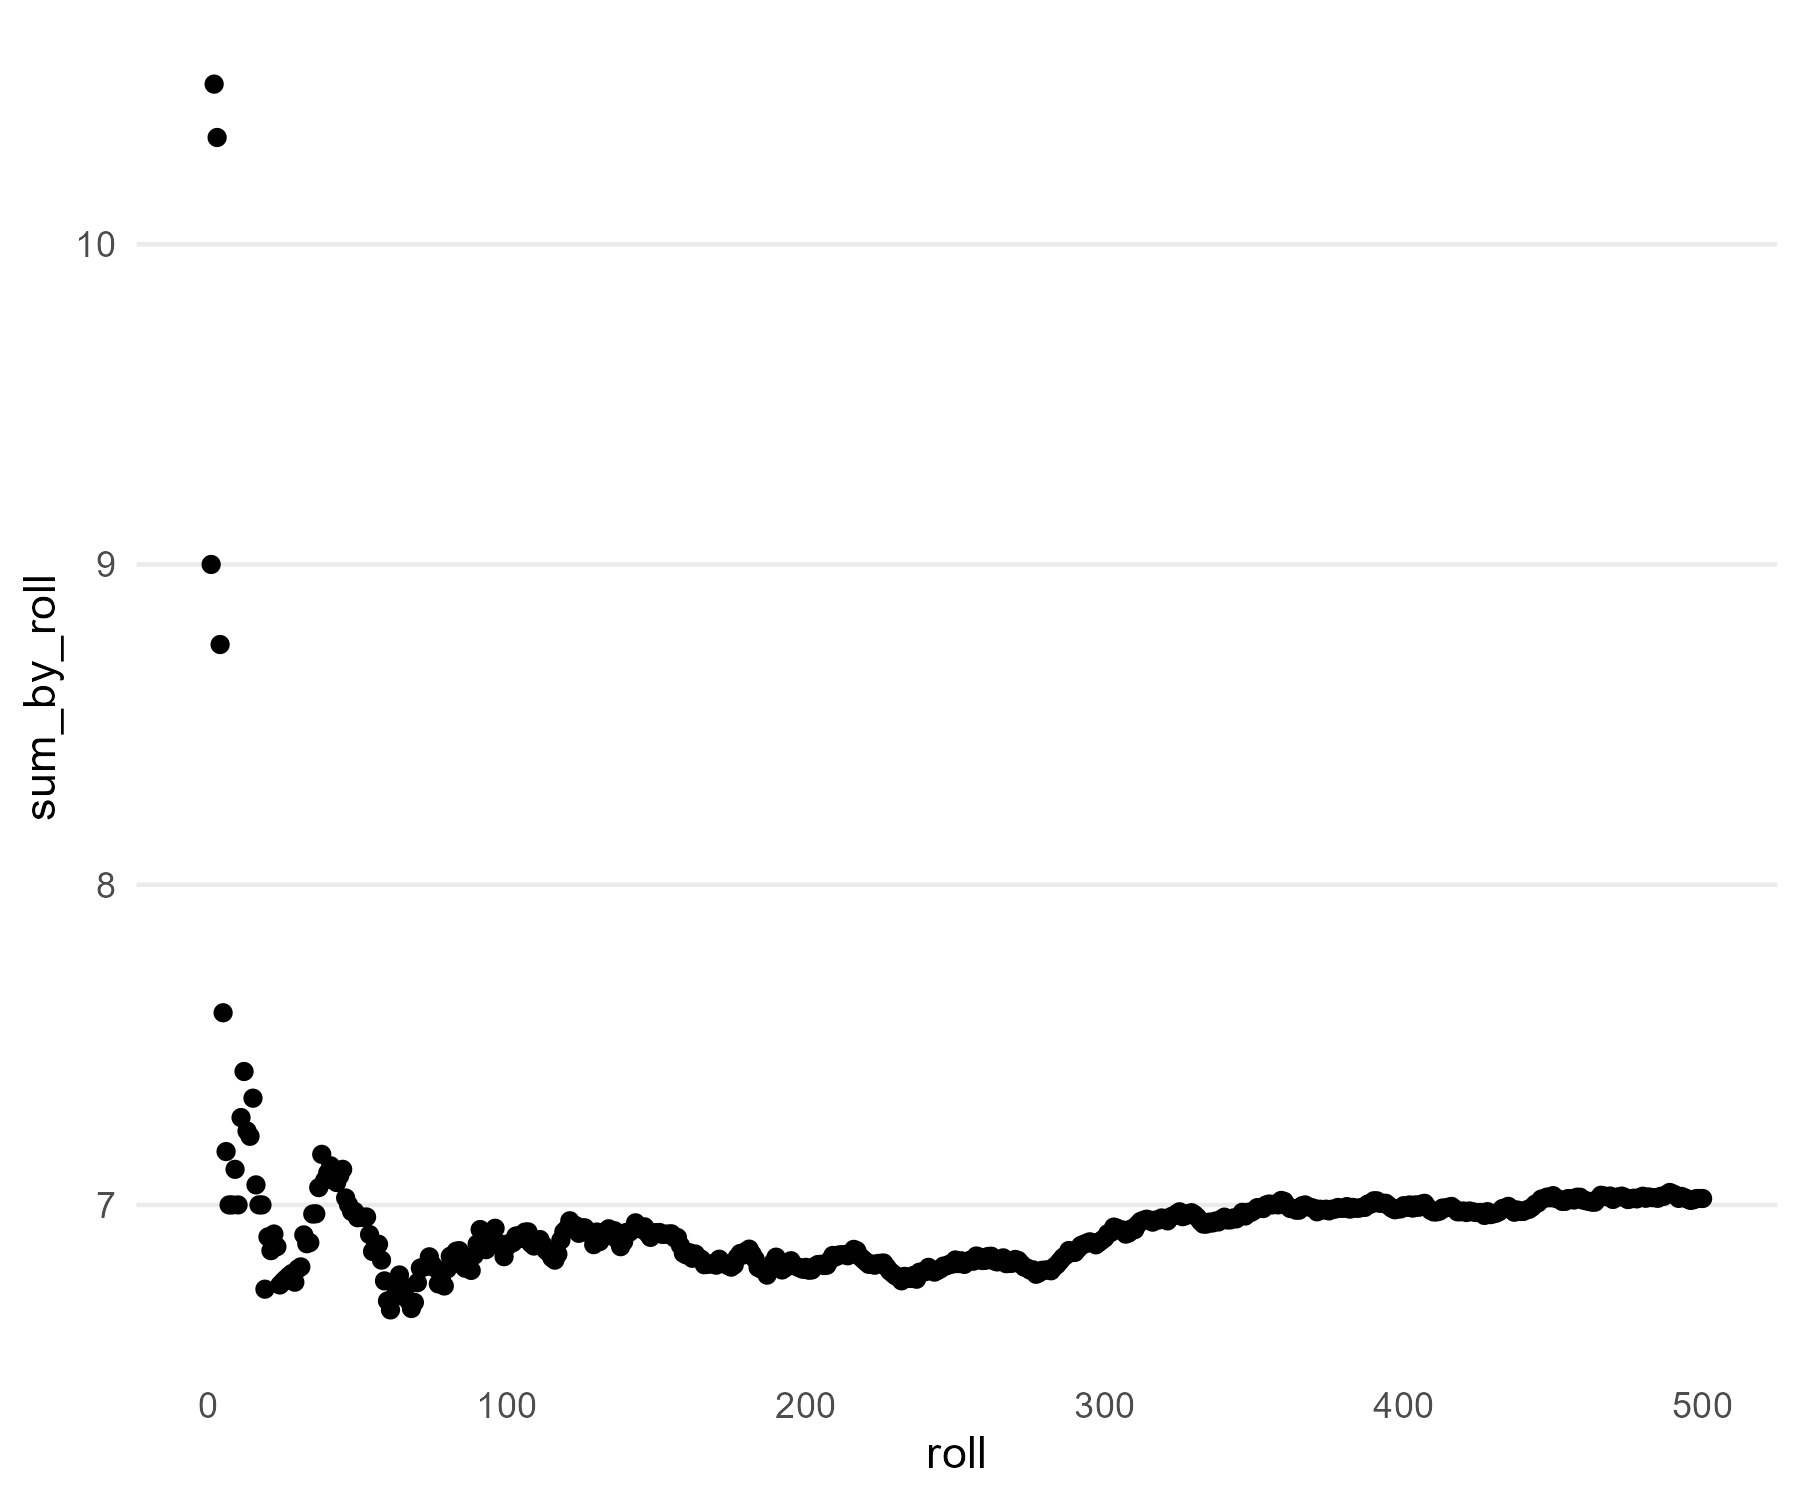
\includegraphics[width=.8\linewidth]{plot/baseline/lln_plot_baseline.png}
\caption[]{Mean for the sum of two six-sided die. Figure based on \input{../../analysis/output/simulation/baseline/sample_size.txt}throws. Approaches value of \input{../../analysis/output/simulation/baseline/mean_sum.txt}}
\label{fig:scatter_baseline}
\end{figure}

\newpage

We also include a second simulation for an 8-sided dice. The corresponding scatterplot is depicted in Figure 
\ref{fig:scatter_8side} 
\begin{figure}[tbh!]
\centering
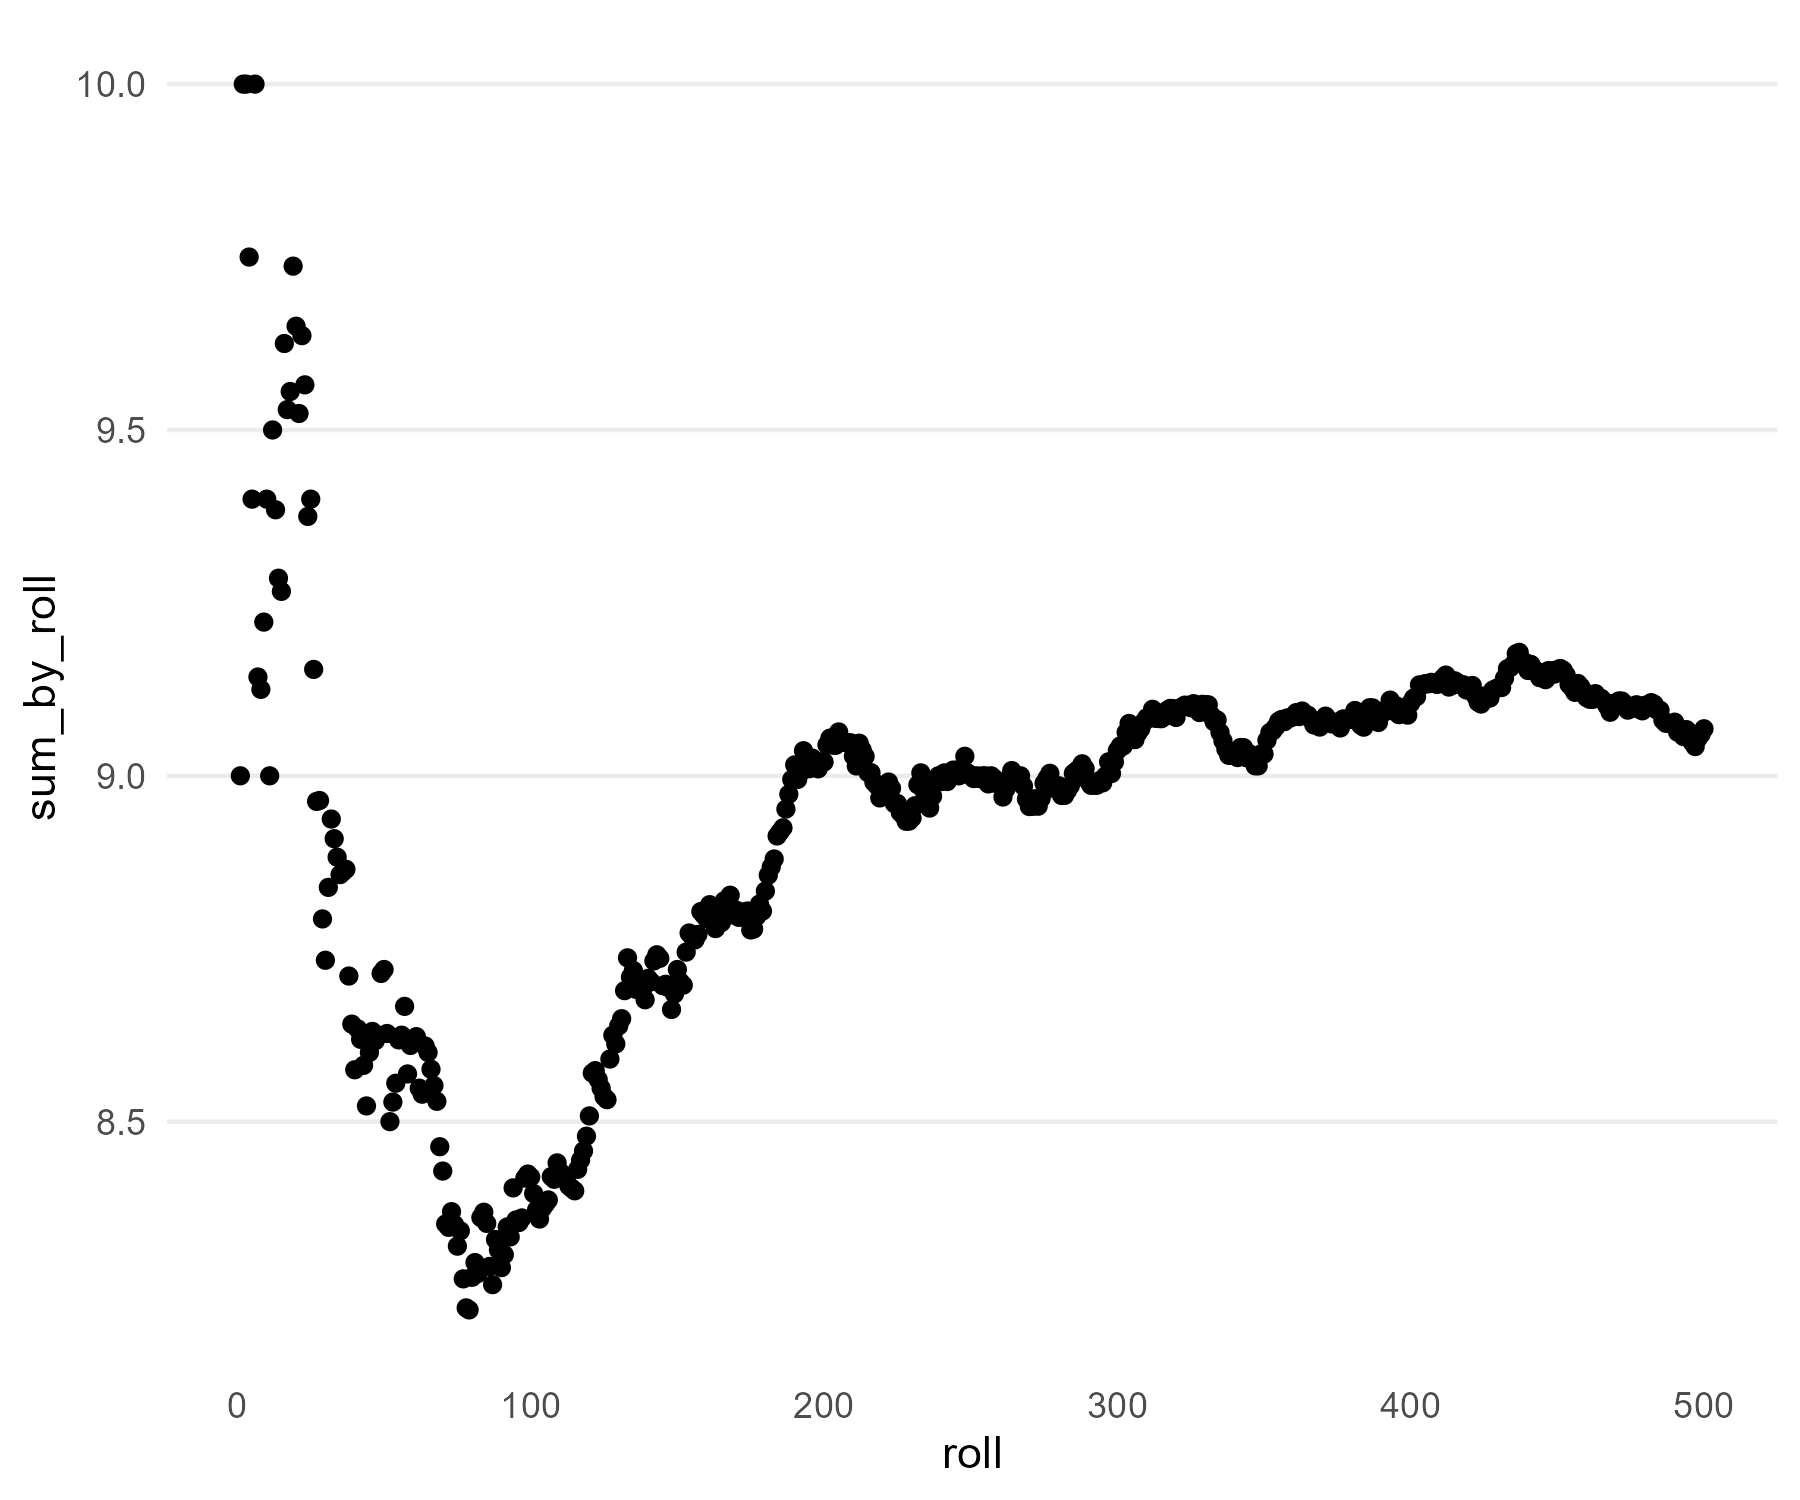
\includegraphics[width=.8\linewidth]{plot/500_8/lln_plot_500_8.png}
\caption[]{Mean for the sum of two eight-sided die. Figure based on \input{../../analysis/output/simulation/500_8/sample_size.txt}throws. Approaches value of \input{../../analysis/output/simulation/500_8/mean_sum.txt}}
\label{fig:scatter_8side}
\end{figure}

\newpage

This is Figure \ref{fig:figsubplots2} with both of the previous scatterplots as subplots. 
\begin{figure}[tbh!]
\begin{subfigure}{.5\textwidth}
  \centering
  % include first image
  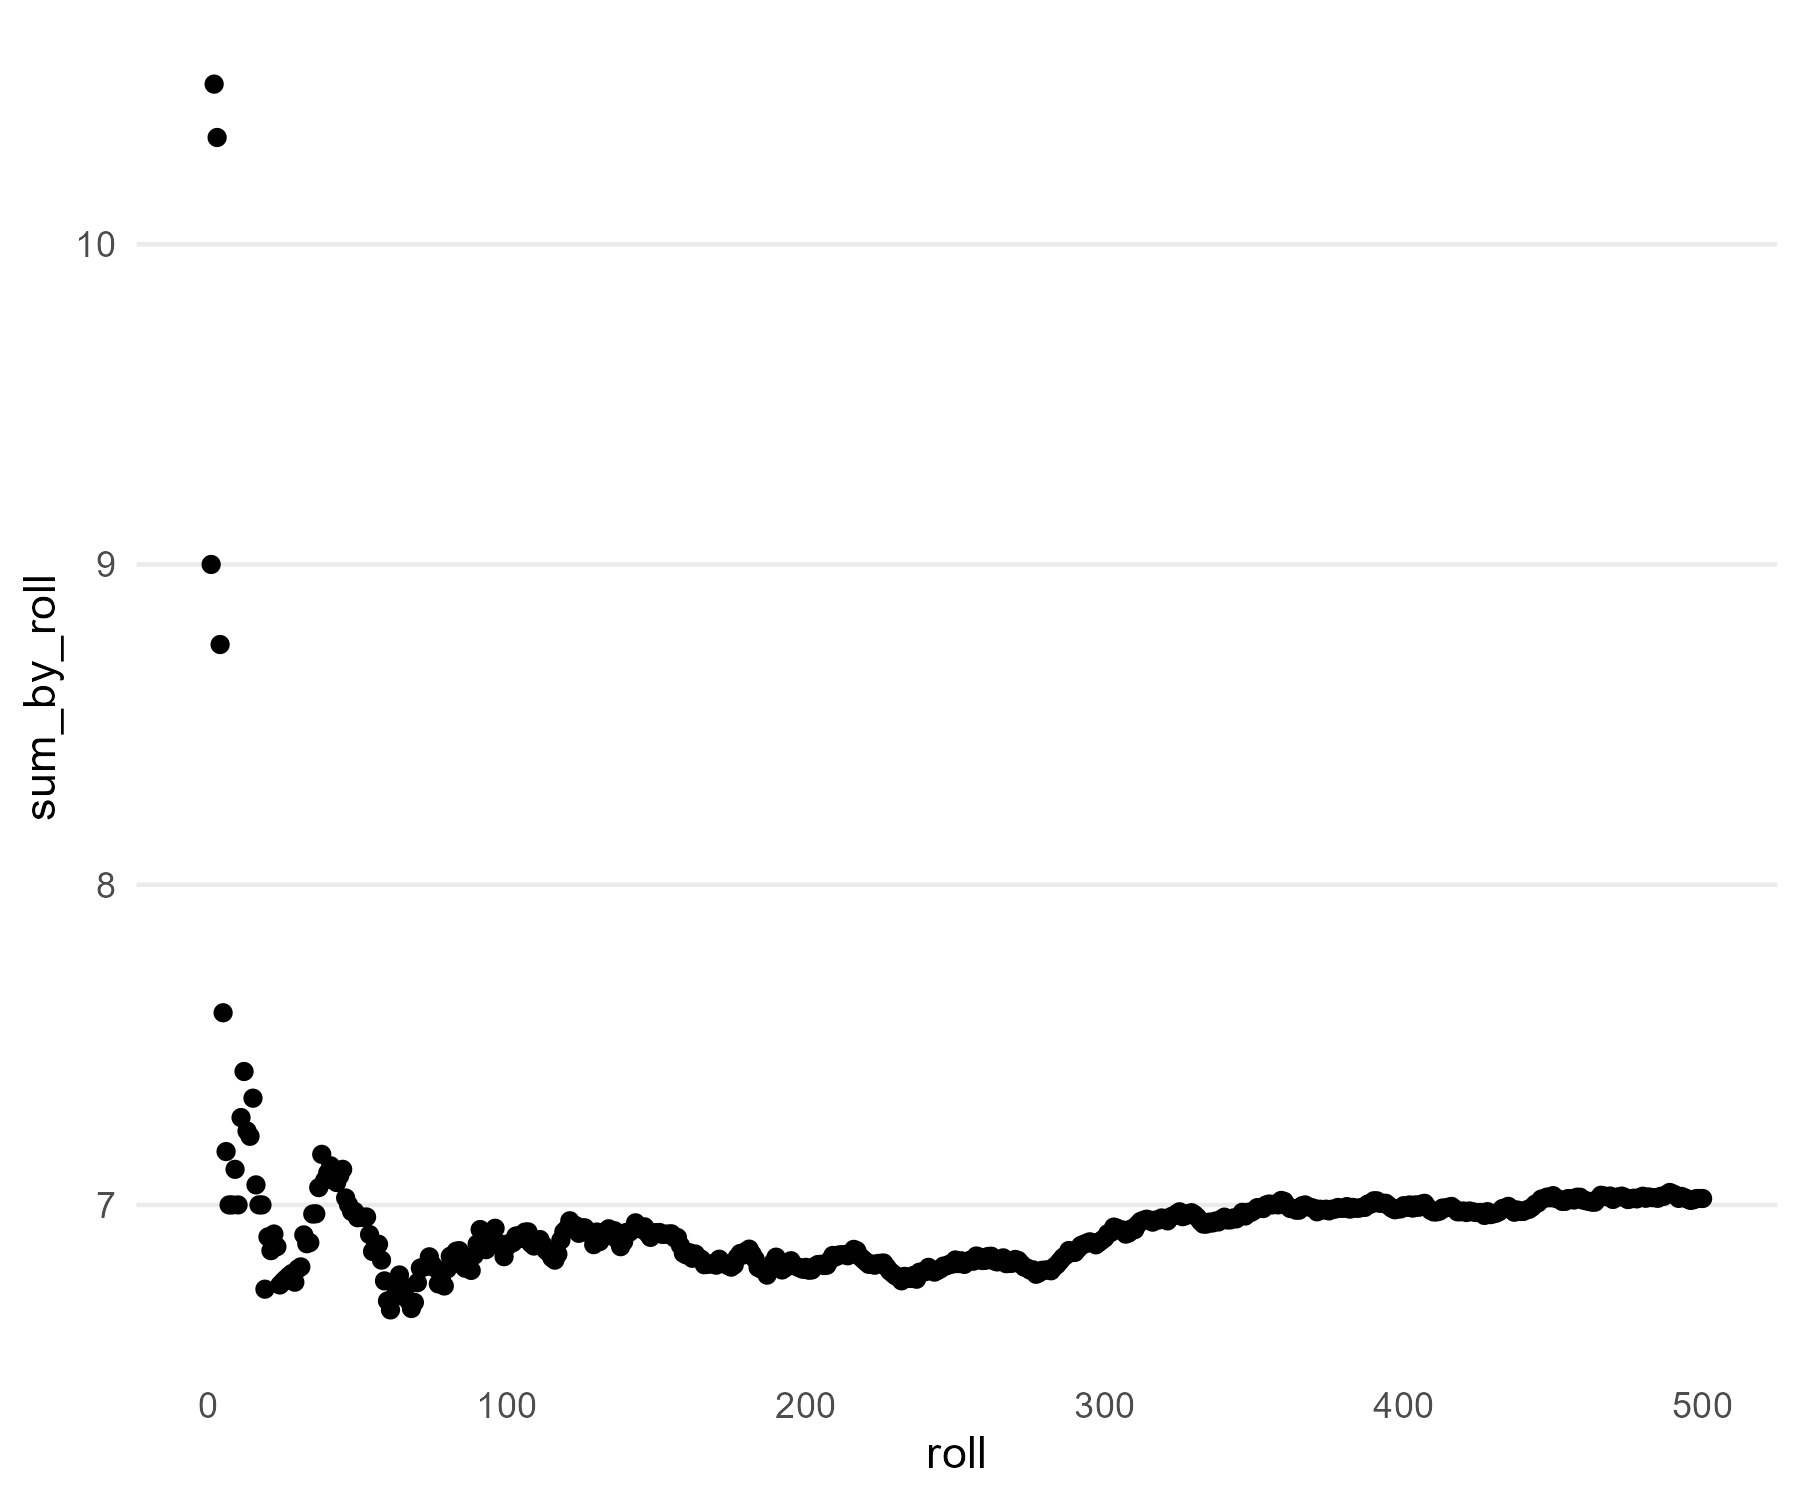
\includegraphics[width=0.8\linewidth]{plot/baseline/lln_plot_baseline.png}  
  \caption{Mean for the sum of two six-sided die. Figure based on \input{../../analysis/output/simulation/baseline/sample_size.txt}throws.}
  \label{fig:sub-first2}
\end{subfigure}
\begin{subfigure}{.5\textwidth}
  \centering
  % include second image
  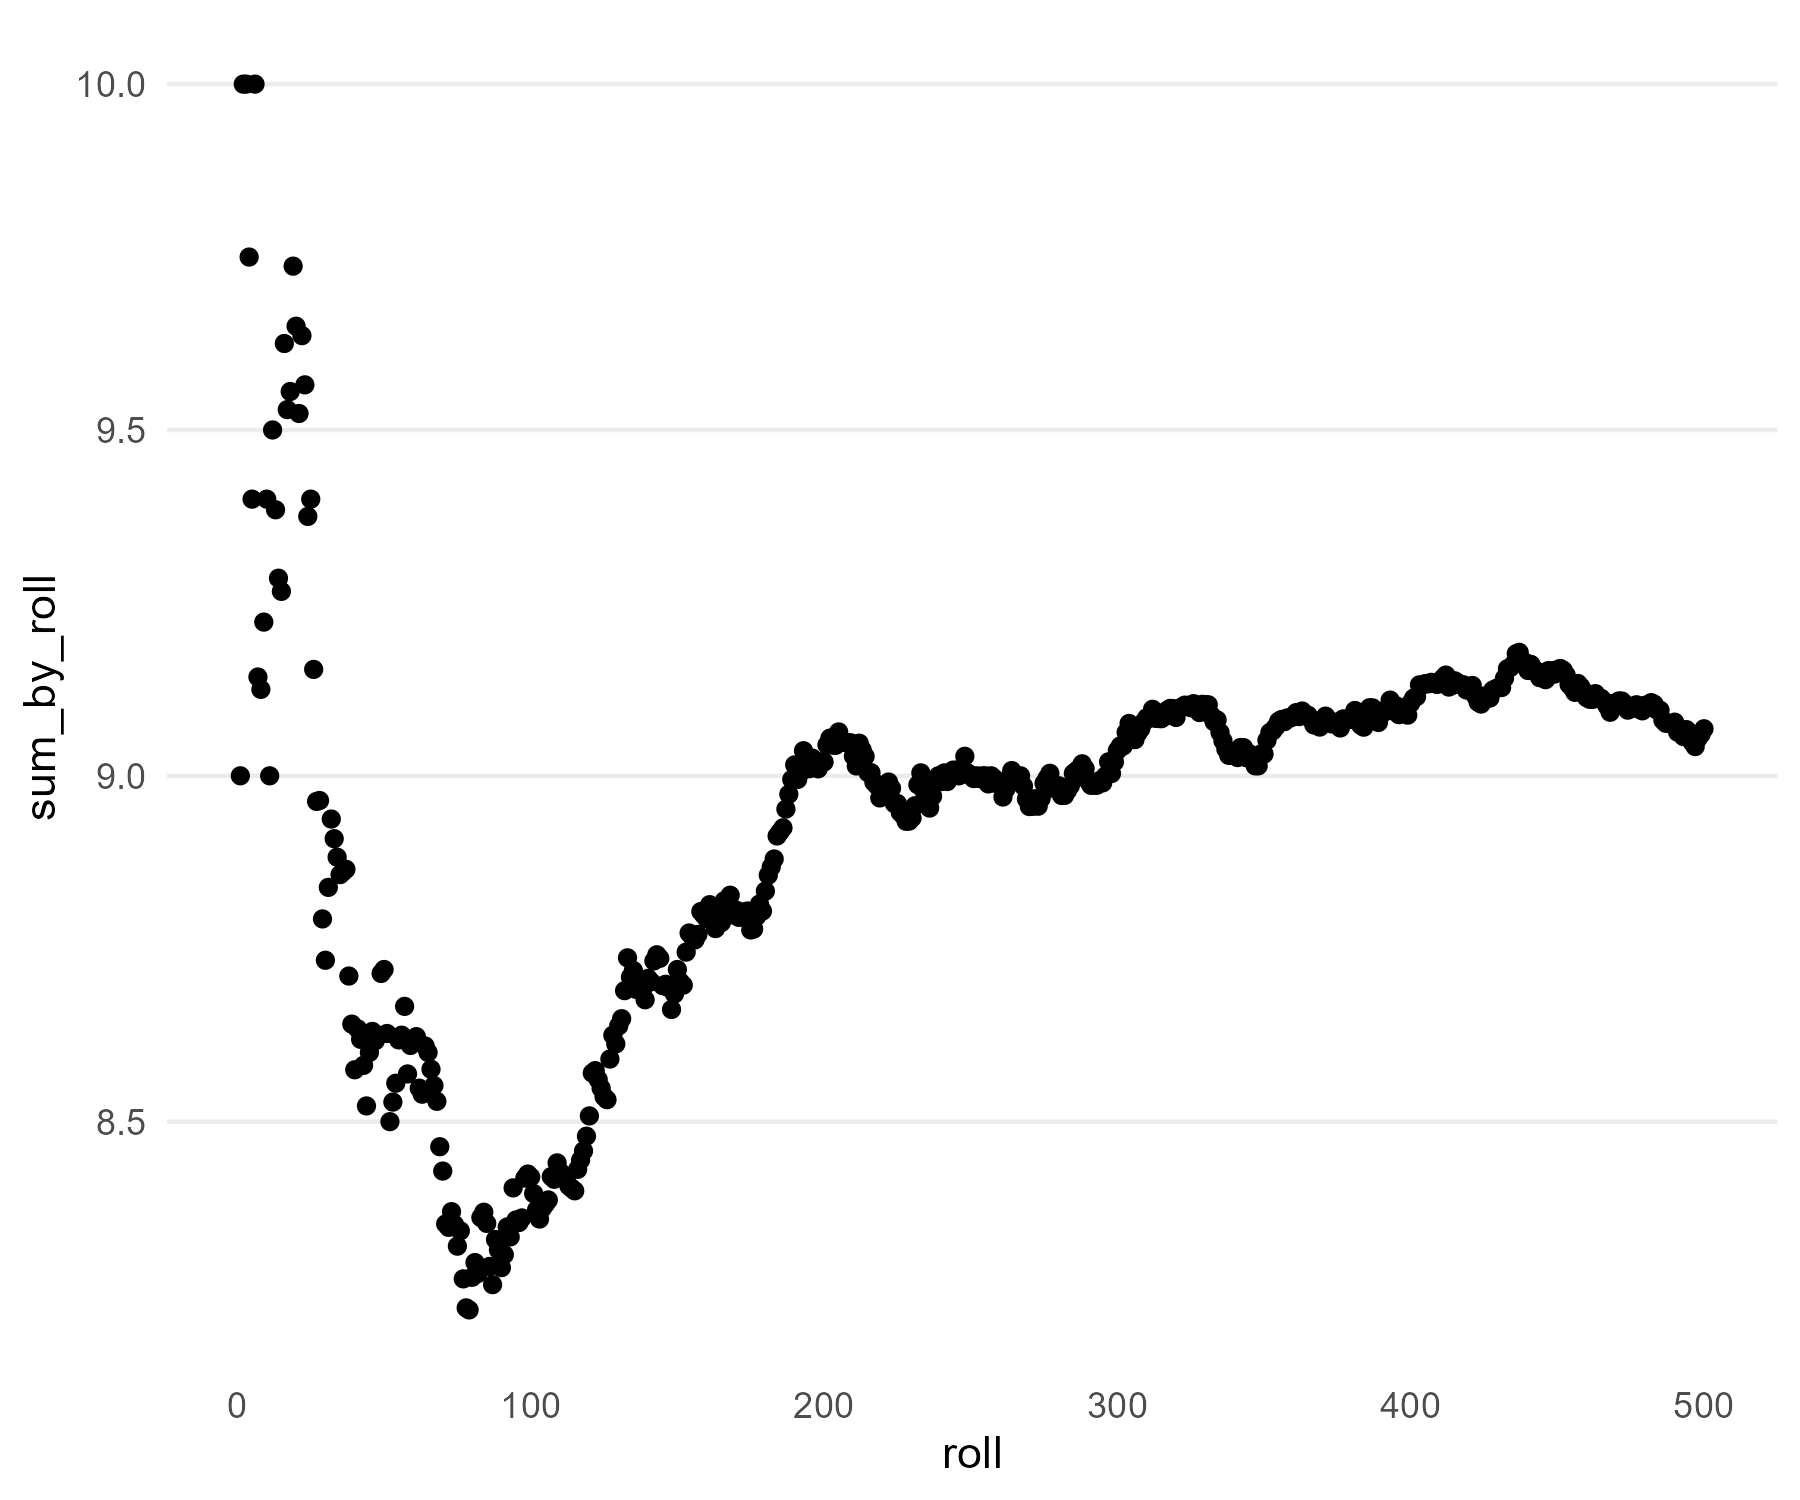
\includegraphics[width=0.8\linewidth]{plot/500_8/lln_plot_500_8.png}  
  \caption{Mean for the sum of two eight-sided die. Figure based on \input{../../analysis/output/simulation/500_8/sample_size.txt}throws.}
  \label{fig:sub-second2}
\end{subfigure}
\caption{Combined plots of the simulations.}
\label{fig:figsubplots2}
\end{figure} \\[12pt] 

Finally, we add a scatter plot from an exemplary do file in Stata in Figure \ref{fig:auto_scatter}.
\begin{figure}[tbh!]
\centering
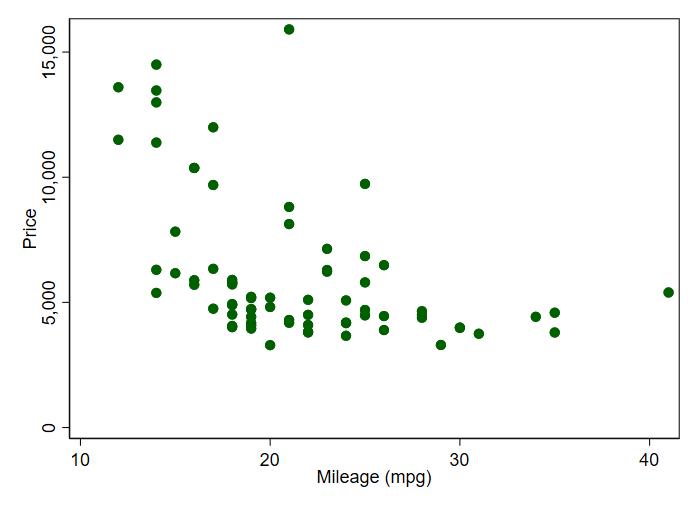
\includegraphics[width=.6\linewidth]{application/scatter.png}
\caption[]{Stata example}
\label{fig:auto_scatter}
\end{figure}

\newpage 

%=======================================================
\bibliographystyle{plainnat}
\bibliography{example}
%\addbibresource{bib_fairness_mc}

%=======================================================

\end{document}


